\documentclass{standalone}
\usepackage{tikz}
% \usepackage{pgfmath}

\usepackage{calc}
\usetikzlibrary{intersections, calc}
\usepackage{hsbcommon}

% \def\myopacity{1}
    \begin{document}

% \def\myopacity{1}
    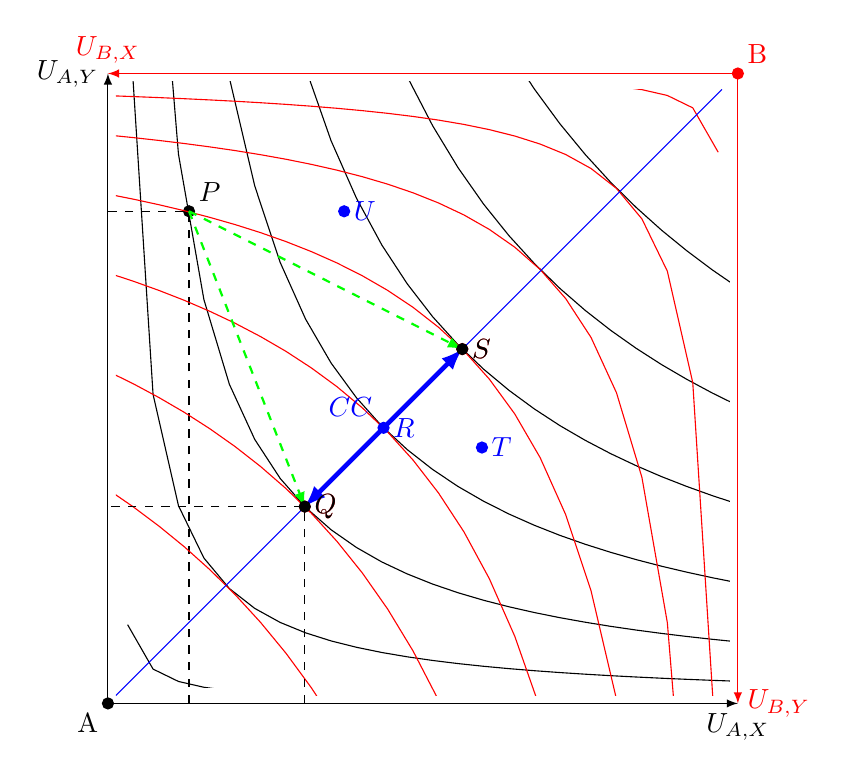
\begin{tikzpicture}[domain=0:8]
        \begin{scope}
                
            \draw[->,>=latex] (0,0) node[below left] {A} -- (8,0) node[below]  {$U_{A,X}$};
            \draw[->,>=latex] (0,0) -- (0,8) node[left]  {$U_{A,Y}$};
            \filldraw (0,0) circle (2pt);

            \ifstep{2}{
\begin{scope}[color=red]

                
                \draw[->,>=latex] (8,8) node[above right]{B}  -- (8,0) node[right]  {$U_{B,Y}$};
                \draw[->,>=latex] (8,8) -- (0,8) node[above]  {$U_{B,X}$};
                \filldraw (8,8) circle (2pt);
            \end{scope}
}

        
            \coordinate (P) at (1.03,6.25); 
            \draw[dashed] (P |-,0) -- (P) -- (0,|- P);
            \filldraw  (P) circle (2pt) node [above right] {$P$};
    
            \clip (0.2,0.2) rectangle (7.9,7.9);
            
            \def\myalpha{0.5}
            \def\mybeta{0.5}
            \def\myfaktor{1}
            \def\myprice{0.5}
            \def\mycolor{black}
    
            \foreach [count=\i] \niveau in {0.5,1.5,...,7}
                {
                \draw[domain=0.25:8, name path=a\i,color=\mycolor] plot (\x, {(\myfaktor*\niveau)/\x^\myalpha)^(1/\mybeta)}); 
                }
    
        \end{scope}
        \begin{scope}[xshift=8cm,yshift=8cm]
            \ifstep{2}{
\begin{scope}[rotate=180,color=red]

                \clip (0.2,0.2) rectangle (7.9,7.9);
    
            \def\myalpha{0.5}
            \def\mybeta{0.5}
            \def\myfaktor{1}
            \def\myprice{0.5}
            \def\mycolor{red}
    
                
            \foreach [count=\i] \niveau in {0.5,1.5,...,7}
                {
                % \pgfmathparse{int(mod(\i,5))}% mod 5 => every fifth
                % \edef\mycolor{\ifnum\pgfmathresult=3 green\else white\fi}
                \draw[domain=0.25:8, name path=b\i,color=\mycolor] plot ({(\x)}, {(\myfaktor*\niveau)/\x^\myalpha)^(1/\mybeta)}); 
                }
    
    
    
                \coordinate (Q) at (5.5,5.5); 
                \filldraw  (Q) circle (2pt) node [right] {$Q$};
                \coordinate (S) at (3.5,3.5); 
                \filldraw  (S) circle (2pt) node [right] {$S$};
    
                \draw[blue] (0,0) -- (8,8);
            \end{scope}
}

        \end{scope}
        \ifstep{2}{\draw[dashed] (Q |-,0) -- (Q) -- (0,|- Q);}

        \ifstep{3}{
\begin{scope}[color=green]

            \draw[dashed,->,>=latex,thick] (P) -- (Q);
            \draw[dashed,->,>=latex,thick] (P) -- (S);
        \end{scope}
}

        \ifstep{4}{
\begin{scope}[color=blue]

                \coordinate (R) at (3.5,3.5); 
                \filldraw  (R) circle (2pt) node [right] {$R$};       
                \coordinate (T) at (4.75,3.25); 
                \filldraw  (T) circle (2pt) node [right] {$T$};
                \coordinate (U) at (3,6.25); 
                \filldraw  (U) circle (2pt) node [right] {$U$};
            \draw[<->,>=latex, ultra thick] (Q) -- node [above left] {$CC$} (S);
            \filldraw[black]  (Q) circle (2pt) node [right] {$Q$};
            \filldraw[black]  (S) circle (2pt) node [right] {$S$};
        \end{scope}
}

    \end{tikzpicture}
\end{document}